\section{Figuras y otros entornos}
\label{sec:figuras}
En éste capítulo hay ejemplos de como poner figuras.
La manera más común es que las figuras aparezcan centradas junto con su pie de figura.
Aceptan los \href{https://en.wikibooks.org/wiki/LaTeX/Floats,_Figures_and_Captions#Figures}{modificadores de posición} usuales.
Lo mas común es usar \mintinline{latex}{[htc]}
 
\begin{figure}[htb]
  \centering
  \label{fig:normalDist}
  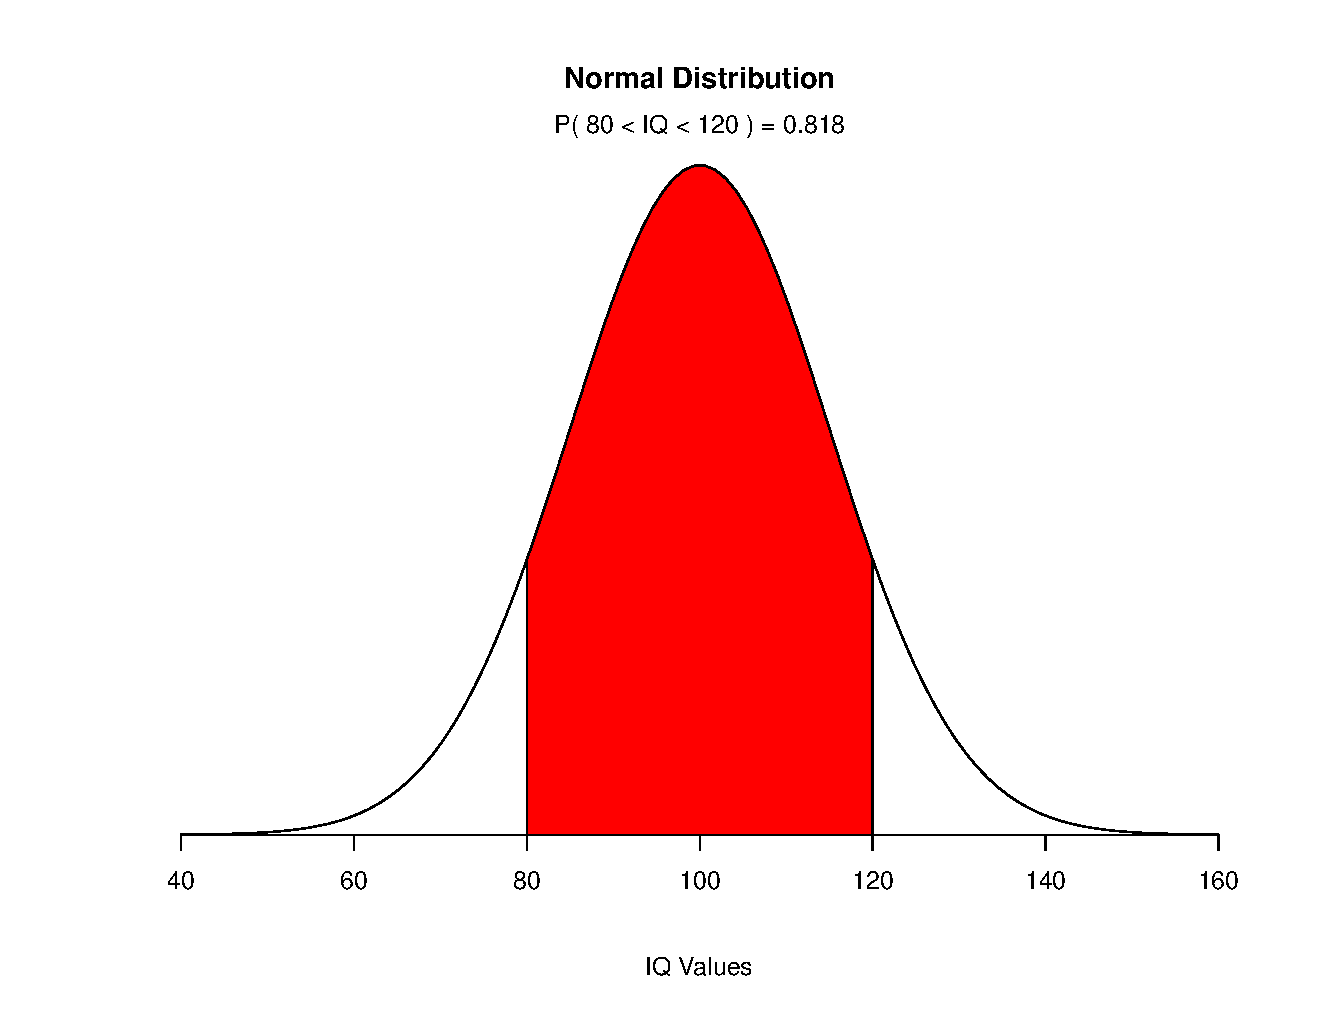
\includegraphics[width=0.85\textwidth]{img/02/normal}
  \caption[Distribución normal]{Gráfica de una distribución normal. Fue creado usando el siguiente \href{https://www.statmethods.net/advgraphs/probability.html}{script en R}.}
\end{figure}

Por regla general, lo mejor es usar imágenes de tipo vectorial.
Mi tipo de formato preferido es \verb|*.eps| y recomiendo usar \href{https://ipe.otfried.org/}{IPE} o \href{https://inkscape.org/}{InkScape}, pero otros formatos vectoriales populares para imágenes son el \verb|*.pdf| y \verb|*.svg|.

\subsection{Subfiguras}

También es posible poner figuras, compuestas de varias subfiguras.
Cada subfigura tiene su propio pié y hay un pié de fígura extra para todo el grupo.
Posteriormente, es posible referirse a toda la figura así: Véase la  Figura~\ref{fig:two} ó referirte a una subfigura así:
Vea la Sub Fígura~\ref{fig:2b}.

\begin{figure}[htp]
 \centering
 \begin{subfigure}[b]{0.45\textwidth}
   
\includegraphics[width=\textwidth]{img/02/ambiente}
   \caption{Componente de reflexión ambiental.}
 \label{fig:2a}
 \end{subfigure}
~
 \begin{subfigure}[b]{0.45\textwidth}
   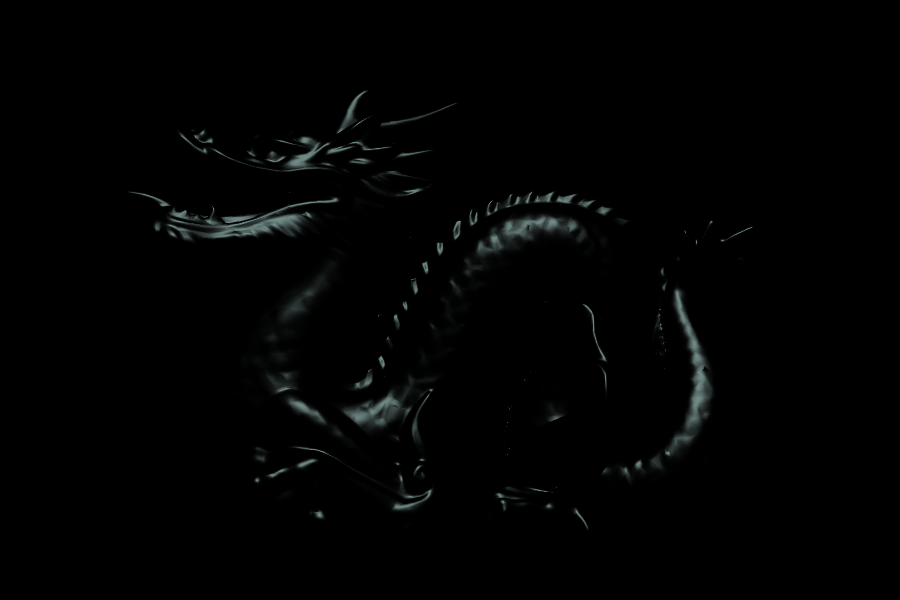
\includegraphics[width=\textwidth]{img/02/especular}
   \caption{Componente de reflexión especular.}
   \label{fig:2b}
 \end{subfigure}
\\
 \begin{subfigure}[b]{0.45\textwidth}
   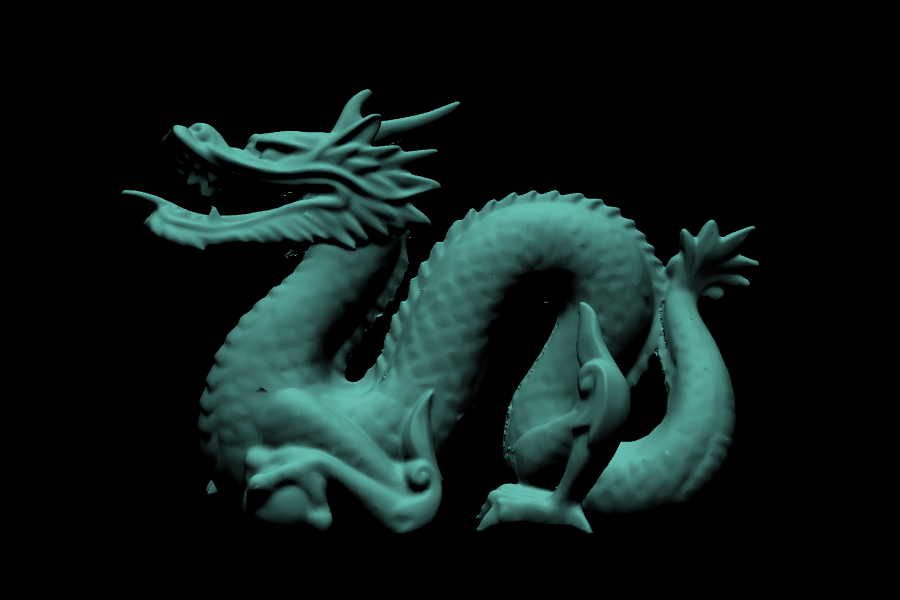
\includegraphics[width=\textwidth]{img/02/difuso}
   \caption{Componente de reflexión difuso.}
   \label{fig:2c}
 \end{subfigure}
~
 \begin{subfigure}[b]{0.45\textwidth}
   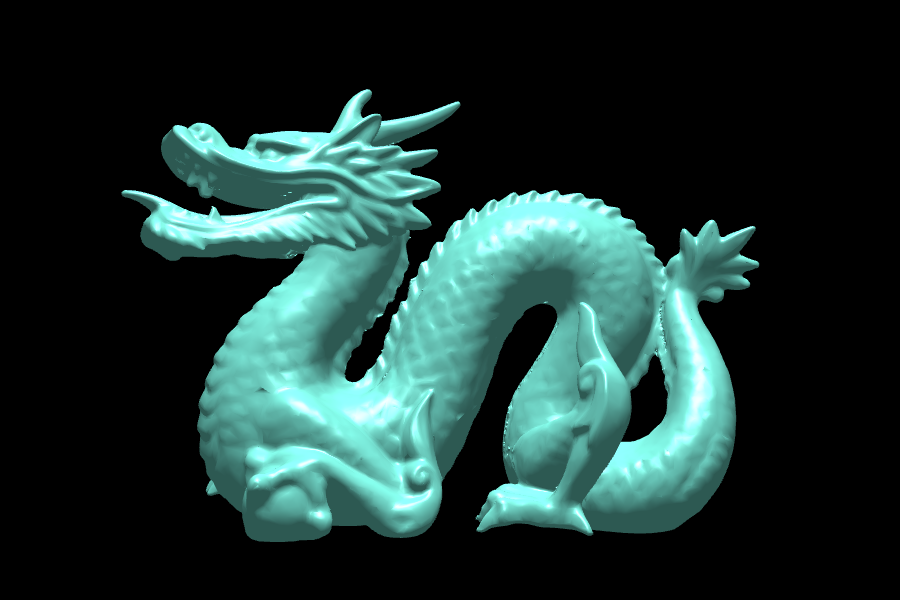
\includegraphics[width=\textwidth]{img/02/completo}
   \caption{Modelo completo.}
   \label{fig:2d}
 \end{subfigure}
 \caption[Módelo de iluminación de Phong]{Componentes del módelo de iluminación de Phong.}
 \label{fig:two}
\end{figure}

Por regla general usamos entornos flotantes para poner Figuras, Tablas o pedazos de código.
Esto quiere decir que tenemos que usar especificadores como guías para que \LaTeX{} sepa dónde ponerlos exactamente en el texto.
Puedes consultar más de eso en \href{https://en.wikibooks.org/wiki/LaTeX/Floats,_Figures_and_Captions}{este} wikilibro.

Así es como se cita un libro: éste ejemplo fué tomado de~\cite{Gonzalez:ImagenesDigitales}.
También hay un ejemplo de como hacer que un libro aparezca en las referencias sin que esté citado explícitamente en el texto.

Por último, este es un ejemplo de una tabla muy elegante: Cuadro~\ref{tab:exey}.
Hace uso del paquete \href{https://ctan.org/pkg/booktabs}{booktabs} por que las tablas predeterminadas en \LaTeX se ven muy anticuadas.
Debes de consultar este \href{https://jdhao.github.io/2019/08/27/latex_table_with_booktabs/}{post} y leer esta \href{https://people.inf.ethz.ch/markusp/teaching/guides/guide-tables.pdf}{presentacion} si vas a uasr muchas tablas en tu tesis.

\begin{table}[htb]
  \begin{center}
    \begin{tabular}{l | r r r r r}
      \toprule
      Source & \textbf{DF} & \textbf{SS} & \textbf{MS} & \textbf{F} & \textbf{P-value} \\
      \midrule
      \textbf{Modelo} & 2 & 0.00318564 & 0.00159282 & 7.72 & 0.0014 \\
      \textbf{Error} & 42 & 0.00866760 & 0.00020637 &  & \\
      \midrule
      \textbf{Total} & 44 & 0.01185324 &   &  & \\
      \bottomrule
    \end{tabular}
  \end{center}
\caption{Tabla Anova para un ejercicio imaginario}
\label{tab:exey}
\end{table}
